\documentclass[12pt]{report}
\usepackage[utf8]{inputenc}

% Change font
\renewcommand*\rmdefault{ppl}

% Set margins
\usepackage[margin=35mm]{geometry}

% Equations
\usepackage{mathtools}

% Greek text characters
\usepackage{textgreek}

% Gap between paragraphs
\usepackage{parskip}

% Line spacing
\usepackage{setspace}

% URL formatting
\usepackage{hyperref}

% Algorithm formatting
\usepackage{algpseudocode, algorithm}

% Sideways tables
\usepackage{rotating}

% Table cell colouring
\usepackage{colortbl}

% Ticks and crosses
\usepackage{amsfonts}

% Captions over page
\usepackage{ccaption}

% References in table of contents
\usepackage[nottoc,notlof,notlot,numbib]{tocbibind}

% Bold in table columns
\usepackage{array}

% Flowcharts
\usepackage{tikz}
\usetikzlibrary{shapes.geometric, arrows}

% Format figure captions
\usepackage[labelsep=space,font={small}]{caption}
\captionsetup{labelfont=bf}
\setlength{\captionmargin}{20pt}
\setlength{\abovecaptionskip}{10pt}

% Page break after sections
\let\oldsection\section
\renewcommand\section{\clearpage\oldsection}

% Monospaced code blocks
\usepackage{listings}
\usepackage{color}
\definecolor{backcolour}{rgb}{0.95,0.95,0.92}
\lstdefinestyle{lststyle}{
    basicstyle=\scriptsize,
    backgroundcolor=\color{backcolour},
}
\lstset{style=lststyle}

\begin{document}

\begin{titlepage}
\thispagestyle{plain}
{\scshape\Large In-silico guided prediction of allosteric sites on proteins: application to cyclin-dependent kinase 2\par}
\vspace{1.5cm}
{\huge\bfseries Joe G Greener\par}
\end{titlepage}

\onehalfspacing

\begin{abstract}
\thispagestyle{plain}
\setcounter{page}{3}

% 300 word limit
Allostery is the functional change at one site on a protein caused by a change at a distant site.
Despite being discovered more than 50 years ago allostery has remained a mystery, and there is no unified scheme to understand and predict it.
In order for the the benefits of allostery to be taken advantage of, both for basic understanding of proteins and to develop new classes of drugs, computational methods to predict allosteric sites on proteins need to be developed and validated.
This thesis introduces two computational methods to predict allosteric sites on proteins and describes experiments to validate a predicted allosteric site.

The concepts of allostery, allosteric prediction, the protein structural ensemble and protein kinases are introduced.
AlloPred uses perturbation of normal modes alongside pocket descriptors in a machine learning approach that ranks the pockets on a protein in terms of their allosteric character.
AlloPred shows comparable and complementary performance to two existing methods.
The AlloPred web server allows visualisation and analysis of predictions.

ExProSE (Exploration of Protein Structural Ensembles), a distance geometry-based method that generates an ensemble of protein structures from two input structures, is described.
ExProSE is able to access conformational changes inaccessible to classical molecular dynamics.
By adding additional constraints to the method, the effect of allosteric modulators can be predicted.
ExProSE is shown to be effective at allosteric site prediction in a systematic comparison of methods.

A predicted allosteric pocket on cyclin-dependent kinase 2, a medically-important protein kinase involved in cell cycle regulation, is explored experimentally.
Selected compounds from a virtual screen were tested in two assays, though no conclusive results were obtained.
The development and adoption of methods such as those presented here is essential or the long-preached potential of allostery will remain elusive.

\end{abstract}


\setcounter{page}{3}
\chapter*{Acknowledgements}

This project was funded by Biotechnology and Biological Sciences Research Council grant BB/J014575/1.

I would like to thank the many people without whom this work would not have happened.
My supervisor Mike Sternberg always offered support and allowed me to pursue my own ideas.
The whole of the Sternberg group provided discussions and a friendly environment - particularly Ioannis for making the work in Chapter~3 so much better, Suhail for keeping the computers working, Alessia for the kind words, Lawrence and Stefans for the pub chats, and Alex and Matt for the lunches over the years.
My co-supervisor David Mann and his group welcomed me in and taught me how to do experiments - Greg in particular was a great teacher, sorry for all the things I broke.
I had an enjoyable 3 months at BenevolentAI on my industry placement and want to thank everyone there for the opportunity.
Thanks also to my progress review panel, Alfonso De Simone and Matthew Fuchter, my other co-supervisor Alan Armstrong, the Stumpf group, and the open source contributors whose software I used.

I would also like to thank my family and friends, who have been so supportive over the years.
My parents and siblings always believed in me more than I believed in myself.
I have known my school friends for 14 or more years now and they still manage to surprise me.
My uni friends have provided such friendship and good times.
Various sports clubs have provided a very direct form of therapy.
And, to Joanna, for making the last year better with a convincing \textit{p}-value.


\tableofcontents

\listoffigures

\listoftables

\chapter*{Abbreviations}

\begin{tabular}{ >{\bfseries}l l }
ASD      &  AlloSteric Database (\url{http://mdl.shsmu.edu.cn/ASD}) \\
CAP      &  Catabolite activator protein \\
CDK2     &  Cyclin-dependent kinase 2 \\
CSA      &  Catalytic Site Atlas (\url{http://www.ebi.ac.uk/thornton-srv/databases/CSA}) \\
ENM      &  Elastic network model \\
ExProSE  &  Exploration of Protein Structural Ensembles \\
FRET     &  F\"{o}rster resonance energy transfer \\
GPCR     &  G protein-coupled receptor \\
KNF      &  Koshland-N\'{e}methy-Filmer (model of allostery) \\
MD       &  Molecular dynamics \\
MWC      &  Monod-Wyman-Changeux (model of allostery) \\
NMA      &  Normal mode analysis \\
NMR      &  Nuclear magnetic resonance \\
NtrC     &  Nitrogen regulatory protein C \\
PC       &  Principal component \\
PCA      &  Principal components analysis \\
PRS      &  Perturbation response scanning \\
SPE      &  Stochastic Proximity Embedding \\
SPR      &  Surface plasmon resonance \\
SVM      &  Support vector machine \\
TR-FRET  &  Time-resolved F\"{o}rster resonance energy transfer \\
TrpAB    &  Tryptophan synthase \\
\end{tabular}


\chapter{Introduction}
\label{cha:introduction}

This chapter introduces the concepts of allostery in proteins, the protein structural ensemble, normal mode analysis, structural prediction of allostery, protein kinases and cyclin-dependent kinase 2 (CDK2).
Some of this introduction has been written as a review (cite).


\section{Normal mode analysis}




\section{Protein kinases}

Protein kinases regulate almost all aspects of cellular physiology, from proliferation and generation of biomass to gene expression and protein production \cite{Manning2002}.
In addition to medical benefits, regulation of kinase activity in mammalian cells is important in industrial production of biomolecules of high value, for example to prevent apoptosis and maximise yield.
In order to modulate kinase activity we need to develop specific regulators of protein kinase function, a process that is complicated by the conserved catalytic architecture of the huge range of protein kinases found in nature \cite{Muller2015}.
One way to achieve kinase regulation with enhanced selectivity is through isolation of allosteric regulators, as their target sites are likely to be less structurally conserved across the protein kinase family.

A few notable examples have highlighted this potential \cite{Gavrin2013}.
Serine/threonine-protein kinase Chk1 has been the target of high-throughput screening efforts \cite{Converso2009}, leading to the discovery of an inhibitor that binds 13 \AA\ from the active site.
This inhibitor binds largely to the protein surface, with part sliding into a narrow hydrophobic cleft, indicating that unexpected sites on proteins may reveal allosteric properties.
Despite locating the allosteric binding site, the mechanism for inhibition is not currently known \cite{Vanderpool2009}.
Study of the tyrosine-protein kinase Abl1 has revealed an inhibitor that binds far from the ATP binding site \cite{Zhang2010, Yang2011}.
Binding of the modulator leads to changes in structural dynamics at the ATP binding site, preventing the binding of ATP and leading to inhibition.
Other targets for which allosteric modulators have been discovered include the MAP kinases \cite{Comess2011} and CDK2 \cite{Betzi2011}.
Modulators such as these that bind protein kinases at sites removed from the ATP-binding site are known as type IV inhibitors.
The binding sites of the above type IV inhibitors, along with others, are shown on the conserved protein kinase structure in Figure~\ref{fig:kinase_mods}.
Type I inhibitors are directly-competitive with ATP as they target the active conformation.
Type II inhibitors bind to the DFG-out conformation and occupy the ATP-binding site and the surrounding hydrophobic region.
Type III inhibitors bind the hydrophobic cleft adjacent to the ATP-binding site but do not bind the ATP-binding site itself.
A novel class of inhibitors, the type V bisubstrate and bivalent inhibitors, has emerged recently \cite{Lamba2012}.
For example, a bivalent inhibitor was designed for a tyrosine kinase that binds to the ATP-binding site and to the regulatory domain SH3 simultaneously via a linker \cite{Hill2009}.
Such binding is able to have both high selectivity and high affinity.
The recent discovery of such sites and the conserved architecture of the eukaryotic protein kinases suggest there are many allosteric sites, particularly for type IV and type V inhibitors, yet to be discovered.

Numerous examples of allosteric kinases are listed in the AlloSteric Database (ASD) \cite{Shen2016}, a resource set up in 2011 that now contains over 1,400 allosteric proteins and over 70,000 allosteric modulators.
The allosteric proteins in the ASD are those that have experimental evidence for allostery.
The increasing number of entries in this database shows that a large number of proteins have allosteric character, and implies that many proteins have allosteric character yet to be discovered.


\begin{figure}
\centering

\includegraphics[width=\textwidth]{images/kinase_mods}

\caption{Binding sites of known type IV allosteric inhibitors are shown in purple on the cAMP-dependent protein kinase (PKA) structure (PDB ID 1ATP).
The ATP binding site is shown in yellow.
Figure reproduced from Lamba and Ghosh (2012) \cite{Lamba2012}.}

\label{fig:kinase_mods}
\end{figure}


\section{Cyclin-dependent kinase 2}

CDK2 is a protein kinase essential for the G1/S phase transition in the cell cycle \cite{Peyressatre2015}.
It associates with, and is regulated by, cyclins.
It has been a major target of drug discovery efforts due to its essential role.


\chapter{AlloPred}

\section{Materials and Methods}

\subsection{Data selection}

ASBench \cite{Huang2015}, a benchmarking set for allosteric discovery, was used as a source of known allosteric proteins.
The `Core-Diversity set' contains 147 structurally-diverse allosteric sites on 127 proteins from a variety of protein classes such as transferases, hydrolases and transcription factors.
The PDB files, allosteric site data and active site data were obtained for each protein from ASBench.
UniProt \cite{TheUniProtConsortium2015} and the Catalytic Site Atlas \cite{Furnham2014} were used to find active site data when it was not available from ASBench.
In each PDB file, only the chain(s) containing the active and allosteric sites, and any chains linking them, were considered.
This was in order to keep the size of the proteins manageable, as using entire protein assemblies would lead to a large number of pockets.
It also allowed comparison with existing methods, which use similar criteria.
In practise the use of larger assemblies was tried during development and did not have a large effect on the results.
7 proteins were removed from the set as the PDB file did not contain the active site, i.e.\ the PDB file represented the allosteric section of a larger protein.
1 protein was removed as Fpocket did not run successfully.
This left 119 proteins in the dataset.
The dataset was randomly split into a training set of 79 proteins and a test set of 40 proteins.


\subsection{Pocket prediction}

Potential binding pockets on the proteins were calculated using the open-source Fpocket v2.0 algorithm, which has been shown to be effective in comparison to other methods \cite{LeGuilloux2009}.
The default parameters used in the Fpocket calculation produced pockets that were large enough to place most (average 86\%) allosteric binding residues in pockets but not so large that identifying a pocket as having allosteric effect was of little use.
Sometimes multiple allosteric pockets on the same protein represented different and physically-separated allosteric sites, and sometimes adjacent calculated pockets covered a single allosteric binding site.
The pockets also covered much of the protein surface, which allowed the method to detect allosteric sites that could be found anywhere on the surface.
On average 41\% of residues in each protein appeared in a pocket.

Fpocket output 2,201 pockets for the 119 proteins (average 18.5 per protein), of which 389 (18\% of pockets, average 3.3 per protein) contained at least one residue identified as binding to an allosteric modulator and were hence labelled as \emph{allosteric pockets}.
Although being defined as an allosteric pocket in this manner does not necessarily mean that binding to that pocket causes the allosteric effect, the average number of allosteric binding residues in an allosteric pocket was 4.3, indicating the utility of locating such pockets.
All but 5 proteins in the dataset had at least one allosteric binding residue placed in a pocket.
We treated pockets without known allosteric binding residues as negative examples during machine learning.
It should be noted that these pockets may not correspond directly to the actual pockets on the protein, or may have latent allosteric character yet to be discovered.


\subsection{Normal mode analysis}

In NMA the Hessian matrix - the matrix of second derivatives of the potential energy $V$ with respect to the mass-weighted atomic coordinates - is diagonalised to yield the normal modes \cite{Hayward2008}.
The potential energy $V$ was described according to the elastic network model \cite{Tirion1996} as a set of harmonic springs of strength $k$ between every pair of C-alpha atoms no further than distance $R_{c}$ apart:
$$
V = \sum_{\substack{r_{ij}^{0} < R_{c} \\ i < j}} k (r_{ij} - r_{ij}^{0})^{2}
$$

where $r_{ij}^{0}$ is the Euclidean distance between atoms $i$ and $j$ in the PDB file.
We used values of 1 kcal mol\textsuperscript{-1} \AA\textsuperscript{-2} and 15 \AA\ for $k$ and $R_{c}$ respectively.

The reduction in flexibility of an allosteric pocket on modulator binding is shown in Figure~\ref{fig:ligand_binding}.
To model this, the unperturbed normal modes were first calculated for the protein.
The calculation was then repeated, each time perturbing one of the pockets in the protein.
If either atom $i$ or $j$ was in the pocket to be perturbed then a higher value of 1.5 kcal mol\textsuperscript{-1} \AA\textsuperscript{-2} for $k$ (1.5 times the previous value) was used instead.
This higher value was chosen after values from 1.2 to 2.5 kcal mol\textsuperscript{-1} \AA\textsuperscript{-2} were examined.
Active site residues were not counted as being in any pocket for this alteration of $k$, in order to avoid direct perturbation of the site at which the effect was measured.
This approach assumes nothing about the shape of the modulator other than that it affects the flexibility of the whole pocket to which it binds.

Once the perturbed NMA had been carried out, the degree of change caused by the perturbation needed to be measured.
Since changes at the active site will likely determine how strong an effect a modulator has, the effect of the perturbation on the active site should be considered.
Within each individual normal mode the effect of the perturbation was measured by averaging across all identified active site residues the magnitude of the difference between the perturbed and the unperturbed displacements from equilibrium.
This is given by:
$$
v_{i} = \frac{1}{N_{a}} \sum_{j=1}^{N_{a}} \left | \mathbf{p_{j}} - \mathbf{u_{j}} \right |
$$

where $v_{i}$ is the effect of the perturbation in normal mode $i$, $\mathbf{p_{j}}$ is the displacement of residue $j$ in the perturbed normal mode, $\mathbf{u_{j}}$ is the displacement of residue $j$ in the unperturbed normal mode, and $N_{a}$ is the number of active site residues.

The effects of the perturbation within each normal mode then needed to be averaged across the modes in order to get a single numeric measure for the strength of the effect arising from perturbation at one pocket.
The effect within each of the normal modes was weighted by the frequency such that the lowest-frequency mode of the chosen modes had the greatest influence on the results.
The equation to determine the effect of a perturbation $C_{m}$ is:
$$
C_{m} = \sum_{i=1}^{m} \frac{v_{i}}{\omega_{i}}
$$

where $v_{i}$ is defined above, $\omega_{i}$ is the frequency of mode $i$ and is hence equal to the square root of the eigenvalue $E_{i}$, and $m$ is the number of normal modes chosen for the calculation.
The justification for this method was that lower-frequency modes within the range selected are likely to be more important in allosteric communication because they consist of the long-range motions of many atoms \cite{Rodgers2013}.

It might be expected that larger pockets will have a higher $C_{m}$ value simply by virtue of having more residues perturbed.
In order to account for this a second measure, $E_{m}$, was defined as:
$$
E_{m} = \frac{C_{m}}{N_{p}}
$$

where $N_{p}$ is the number of residues in the pocket and $C_{m}$ was defined previously.
$E_{m}$ is a measure of the amount of change caused at the active site per residue in the perturbed pocket.
A Python script utilising the ProDy package \cite{Bakan2011} was used to perform NMA on the proteins.


\subsection{Machine learning}

Values of $C_{m}$ and $E_{m}$ with $m$ equal to 20, 50, 100, 200 and all modes were chosen as features in a SVM.
The features from the Fpocket output used in the SVM were:
\begin{itemize}
\item Rank
\item Score
\item Druggability score
\item Number of alpha spheres
\item Total SASA
\item Polar SASA
\item Apolar SASA
\item Volume
\item Mean local hydrophobic density
\item Mean alpha sphere radius
\item Mean alpha sphere solvent accessibility
\item Apolar alpha sphere proportion
\item Hydrophobicity score
\item Volume score
\item Polarity score
\item Charge score
\item Proportion of polar atoms
\item Alpha sphere density
\item Centre of mass - alpha sphere max distance
\item Flexibility
\end{itemize}

See the Fpocket documentation for more details on each of these measures.
Distance to the active site, number of residues in the pocket and number of pockets in the protein were also used as features.
The distance to the active site for each pocket was calculated as the distance between the geometric centre of the active site residues and the geometric centre of the residues in the pocket.
Each feature (apart from number of pockets) was utilised in two different ways: the feature value normalised across all proteins (\emph{raw}); and the ranking of the feature value within the values for that protein, where the ranks were scaled between 0 and 1 (\emph{ranked}).

The 65 features were ranked in Weka explorer \cite{Frank2004} using the ChiSquared attribute evaluator and the Ranker search method.
This evaluates the worth of a feature by computing the value of the chi-squared statistic with respect to the class.
The top 7 features only were retained, as features below this added little value.
The retained features, in descending order of descriptive power, were:
\begin{itemize}
\item Number of alpha spheres (raw)
\item $E_{200}$ (ranked)
\item Score (raw)
\item $E_{all}$ (ranked)
\item Distance to active site (raw)
\item Pocket size (raw)
\item Fpocket rank (raw)
\end{itemize}

The SVM-Light package \cite{Joachims1998} was used to run the SVM.
The Gaussian kernel was selected, containing internal parameters $C$ and $\gamma$.
The cost factor by which training errors on positive examples outweigh errors on negative examples was set as the ratio of negative to positive examples in the training set (6.19).
A leave-one-out parameterisation procedure was carried out over a grid of parameters with $C$ equal to 0.01, 0.1, 1 or 10 and $\gamma$ equal to $10^{-3}$, $10^{-4}$ or $10^{-5}$.
The procedure consisted of training the SVM on pockets from 78 of the 79 proteins in the training set and testing on pockets from the one left out.
The process was repeated for each protein in the set.
Performance was similar across the parameter range, with the parameters $C=1$ and $\gamma=10^{-4}$ being selected for the final SVM.
Due to the low number of allosteric pockets on each protein, only the top prediction was chosen as being allosteric.


\subsection{Web server}

A flowchart outlining the process of running a job is shown in Figure~\ref{fig:flowchart}.
The web server was implemented using the Django extension to Python and a SQLite database.
JSmol, a JavaScript implementation of the Jmol package, was used for molecular visualisation.
Bootstrap was used for page styling.
The standalone version of the code runs faster and it is recommended that users who intend to use the method extensively or in batch download the code for local use.


\section{Results}

AlloPred was tested on a test set of 40 known allosteric proteins (see the Methods section for selection criteria).
For each protein AlloPred ranked the pockets and the top ranked pocket was examined.
For 23 of 40 proteins AlloPred ranked top a pocket containing an allosteric binding residue (an \emph{allosteric pocket}), when 18\% of pockets were allosteric pockets.
For 28 of 40 proteins an allosteric pocket was ranked first or second.
The results were compared to two existing methods for allosteric site prediction.
The AlloSite server uses the Fpocket algorithm and a machine learning approach \cite{Huang2013}, whereas the PARS server combines changes in protein flexibility and a structural conservation score \cite{Panjkovich2014}.
The correct predictions made by each method, and the overlap between the methods, are shown in Figure~\ref{fig:results_venn}.
AlloSite ranked an allosteric pocket top in 21 of 40 cases and is suitable for direct comparison to AlloPred as both methods rank pockets from Fpocket.
PARS, however, makes predictions of single points; a point was considered allosteric for our purposes if it was within 10 \AA\ of an allosteric modulator atom in the protein-modulator crystal structure.
It is important to note the different criteria for a correct prediction when considering the results.
PARS ranked an allosteric pocket top in 10 of 40 cases.
Figure~\ref{fig:results_venn} shows that AlloPred compares well to other methods and makes 4 correct predictions that neither of the other methods do.
This suggests that users of other allosteric prediction methods would benefit from the additional use of AlloPred.

In order to reduce the effects of bias during the split of the dataset into training and test sets, the dataset of 119 proteins was additionally split randomly 20 times into training and tests sets of 79 and 40 proteins respectively.
The SVM was then trained on the training set, using the previous parameters, and tested on the test set.
The average number of correct predictions across the 20 runs was 23.6 out of 40.
This shows that the above results used for comparison to other methods are indicative of the performance of the method.


\subsection{Web server}

The AlloPred web server allows users to analyse the prediction results via an intuitive interface.
Users can either input a PDB ID and chain(s) or upload a PDB file.
The active site residues of the protein must be given but there is an option to retrieve this data, if it is available, from the Catalytic Site Atlas \cite{Furnham2014}.
The results page is shown in Figure~\ref{fig:web_results}.
All pockets are displayed in a table with their AlloPred rankings and Fpocket output.
The table can be sorted and filtered by any one or more of the 29 AlloPred and Fpocket features.
The page also allows users to visualise each pocket on the protein in a JSmol window that lets the user to explore the protein and its predicted allosteric sites.
Features include highlighting the active site residues, selecting one of three visualisation options and a JSmol terminal to insert custom commands.
The results, including full details of each pocket, can be downloaded for further analysis as a tab-delimited text file.
The calculation time is fast, with a 400 residue protein ($\sim$15 predicted pockets) analysed within 5 minutes.


\section{Discussion}

Over the last few years a renewed interest in allostery, perhaps due to the potential benefits of allosteric drugs, has led to the development of a number of computational approaches to understanding allostery \cite{Collier2013}.
Some of these are directly associated with predicting allosteric sites on proteins from structure alone.

The AlloSite server is similar to the method presented here in that it uses the Fpocket algorithm and attempts to elucidate allosteric pockets \cite{Huang2013}.
Whereas AlloSite solely uses the Fpocket output, our method uses an approach that combines flexibility with the Fpocket output.
A combination of methods may give better predictions than either method individually, as indicated by the unique predictions made by both methods during testing.
In fact the AlloSite predictions were found in every case to correspond to the pocket ranked top by Fpocket.
The complete ranking of pockets provided by AlloPred may also be useful, as pockets ranked second were often found to be allosteric in the test set.

An approach that combines flexibility analysis using normal modes and structural conservation scores \cite{Panjkovich2012} is also similar to the method presented here and  was recently turned into a web server, PARS \cite{Panjkovich2014}.
Although direct comparison is difficult due to the differences in site calculation, definition of allosteric sites and datasets used, the method presented here again may be used well in combination as shown by Figure~\ref{fig:results_venn}.

The lack of input about the shape of the ligand and the large coverage of the protein in terms of pockets (average 18.5 pockets per protein) used by our method mean that it may be able to predict novel or unusual sites that methods which explicitly model the modulator might not.
This is important, for example when searching for allosteric sites on proteins believed to be non-allosteric.
The lack of conservation-based approaches in our method also facilitates discovery of sites not currently preserved by evolution.
This is useful due to the large variety of allosteric modulators \cite{Wang2012} and mechanisms \cite{Motlagh2014}, suggesting potential novel modulators for proteins with known allosteric pathways.

Other promising approaches \cite{Demerdash2009, Kidd2009, Kaya2013} investigate the allosteric pathway and are not directly comparable with this method, which is only concerned with how the pathways transmit the effects of perturbations to the normal modes and does not directly reveal any information about the pathways themselves.
Again, a combination of our method with these approaches may be useful, as pockets predicted using our or other methods can be further investigated to reveal information about the underlying allosteric communication.

The main limitation of our method is related to the diversity found in allosteric systems.
Rigid-body motions of oligomers, side-chain dynamics, backbone motions and local unfolding are all mechanisms of allostery, with allosteric effects even present in intrinsically-disordered proteins \cite{Motlagh2014}.
A method based around the changes in dynamics on ligand binding is likely to miss many allosteric effects, and this can go some way to explaining the predictions of our method that were incorrect.
In particular, classic examples of allostery such as haemoglobin that involve oligomeric re-organisation to affect ligand cooperativity are not suitable for use with this method.
However, the results shown here and in other studies are encouraging and indicate a future where we can pick modulating sites on proteins with reasonable confidence.
Our method, for example, successfully predicts allosteric sites on proteins with a variety of sizes and functions.


\chapter{ExProSE}

\section{Materials and Methods}

ExProSE is based on the CONCOORD distance geometry method \cite{DeGroot1997}, but has important differences that make it suitable for modelling conformational transitions and ensemble perturbations.
These are primarily the use of two input structures instead of one, a different procedure for achieving convergence, the ability to predict the effect of a modulator and an auto-parameterisation procedure.
ExProSE is implemented in Julia, a language that combines readable syntax similar to Python with performance approaching statically-compiled languages like C.
Use of Julia allows good computational performance at the limiting steps, but also allows compact and easy-to-use code that others can modify.
The code, documentation, details of the datasets and instructions for reproducing the data are freely-available under the MIT license as a Julia package at \url{https://github.com/jgreener64/ProteinEnsembles.jl}.
The code is written in a modular way with associated unit tests and an automated building and testing procedure.


\subsection{Distance constraint generation}

The first step is to obtain a set of distance constraints from a protein structure.
Contrary to similar studies \cite{Panjkovich2012, Huang2013} the smallest biological assembly of the protein is used, rather than only the chain containing the allosteric modulator.
Hetero atom records, including the allosteric modulators, are removed.
Any existing hydrogens are removed and polar hydrogens are added using an in-house script.
Secondary structure assignments, required to obtain additional distance constraints, are obtained using the DSSP software \cite{Touw2015}.
As two structures for the same protein are utilised to generate distance constraints, only atoms common to both structures are used.
Every atom pair is examined and assigned an interaction type.
The criteria for each interaction are the same as in CONCOORD \cite{DeGroot1997} and are shown in Table~\ref{tab:interaction_types}.


\begin{table}
\centering

%\includegraphics[width=\textwidth]{images/interaction_types}

\caption{Interaction types between atom pairs.
These are the same as in CONCOORD \cite{DeGroot1997}.
The constraint tolerance values are used to generate lower and upper distance constraints between atoms.}

\label{tab:interaction_types}
\end{table}


Each atom pair is assigned the first interaction for which it fulfils the criterion.
If an atom pair is not assigned any of the first 14 specific interactions, it is assigned the generic `All other pairs' interaction type.
Lower and upper distance constraints $l_{ij}$ and $u_{ij}$ are generated for each atom pair $ij$ based on the interatomic distance $d_{ij}$, the constraint tolerance for the interaction $t_{ij}$ and a tolerance weighting factor $W_{B}$ that is between 0.0 and 1.0:

$$
l_{ij} = d_{ij} - W_{B} t_{ij}, \quad u_{ij} = d_{ij} + W_{B} t_{ij}
$$

The selection of $W_{B}$ is described below.
For example two atoms 1.54 \AA\ apart and in a covalent bond with $W_{B}$ equal to 0.5 would have a lower distance constraint of 1.53 \AA\ and an upper distance constraint of 1.55 \AA, as the constraint tolerance multiplied by $W_{B}$ is 0.01 \AA.
This process yields a set of distance constraints for each crystal structure of a protein.

The distance constraints generated from the two structures for the same protein are combined to get a set of combined constraints.
The constraints are combined in such a way that the new constraints for a given atom pair cover the distance of both the individual constraints for that pair.
For example if two atoms have a lower and upper distance constraint of 6.0 \AA\ and 7.0 \AA\ in structure one, and 6.5 \AA\ and 7.5 \AA\ in structure two, then the new constraints will be 6.0 \AA\ and 7.5 \AA.

It is undesirable to retain all the `All other pairs' interactions (type 15 in Table~\ref{tab:interaction_types}) as they vastly outnumber the specific interactions (types 1-14).
Specific interactions scale with the atom number $N_{A}$ whereas other pairs scale as $N_{A}^{2}$.
Hence only a fraction of the other pairs are retained as distance constraints.
The probability of retaining an other pair is chosen so that the final number of other pairs is roughly $20N_{A}$, the value used by studies utilising CONCOORD \cite{DeGroot1999}.

$W_{B}$ is chosen for each protein in the apo/holo and allosteric datasets by a process of auto-parameterisation.
$W_{B}$ equal to 0.0 usually results in a narrow range of structures that are midway between the two input structures.
By contrast, $W_{B}$ equal to 1.0 usually results in structures that cover a wide conformational space beyond the input structures.
A measure for the conformational spread of the ensemble was developed.
This measure $F$ is the fraction of structures $S$ in the ensemble for which $TM(S,A) > TM(B,A)$ and $TM(S,B) > TM(A,B)$ where $TM(X,Y)$ is the TM-score between model $X$ and reference $Y$, and $A$ and $B$ are the two input crystal structures.
The TM-score is a measure of similarity between two protein structures.
$F$ therefore gives the proportion of structures that are closer to both input structures than the input structures are to each other.
$F$ equal to 0.9 indicates an ensemble that effectively covers the conformational space of the input structures.
Ensembles of 50 structures are generated with $W_{B}$ starting at 1.0 and decreasing in steps of 0.1.
When the ensemble generated has an $F$ value of at least 0.9, that $W_{B}$ is chosen.
For the specific examples T4-lysozyme and CDK2, $W_{B}$ is equal to 0.2 and 0.3 respectively.
It should be noted that the above auto-parameterisation procedure to select $W_{B}$ is implemented automatically and requires no input by the user.
For CAP only one input structure is used so $W_{B}$ is selected manually as 0.4.
This value allows flexibility in the ensemble whilst giving good quality structures.


\subsection{Protein structure generation}

Once the distance constraints have been generated, an iterative process is used to generate structures that satisfy the constraints.
Stochastic Proximity Embedding (SPE) \cite{Agrafiotis2013} was selected, as it has been shown to converge effectively and scales well with system size.
This procedure provides better convergence than the CONCOORD procedure of moving atoms to a random distance within the distance constraints.
The pseudocode for the SPE algorithm, rephrased from an existing review \cite{Agrafiotis2013}, is shown in Algorithm~S1.
The distance constraints do not include favourability for a particular chirality, so coordinates produced from SPE are examined and structures with the incorrect chirality are reversed by mirroring all coordinates in the $xy$ plane.

Once a set of coordinates has been generated, an SPE error score can be calculated that measures how well the distance constraints are satisfied \cite{Agrafiotis2013}.
This score is calculated as shown in Algorithm~S2.
Structures with a high error score tend to have more violations of allowed stereochemistry, which is to be expected as there are more violations of allowed constraints.
In order to account for this, more structures are generated than required and those with the highest scores are discarded.
The ratio is set to be 1.5.
So if the final ensemble had 200 structures, initially 300 are generated and the 100 with the highest error score are discarded.
This was found during development to generally produce ensembles of structures with acceptable stereochemical quality.

The number of iterations per atom, the product of the number of cycles $C$ and the number of steps $S$ from Algorithm~S1, is taken as 60,000.
This was chosen as the SPE error score did not generally decrease for iterations beyond this.
The ratio of $S$ to $C$ is taken as 50:1 as in practice any value of $S > C$ will give similar results \cite{Agrafiotis2013}.
The reduction in learning rate over the course of the minimisation makes this process similar to simulated annealing.
Initially large movements through the conformational space allow the correct region to be found.
The movements are dampened over time to allow the system to converge to a solution.
This procedure is carried out separately multiple times to obtain an ensemble.


\subsection{Ensemble analysis}

Ensembles of structures produced are iteratively aligned following the procedure described in the methodology of a previous study \cite{Bakan2009}.
This aligns an ensemble without the use of a reference structure.
The average structure of the ensemble is taken as the centroid of the coordinates across the ensemble following this superimposition.

PCA is carried out on the generated ensemble.
The coordinates across the ensemble are compared to the average coordinates and a set of orthogonal motions are found that describe the variation in the ensemble.
The covariance matrix $C_{ij}$ is a matrix where $i$ and $j$ represent the indices of the $3 N_{C}$ atomic coordinates of the $N_{C}$ C\textsuperscript{\textalpha} atoms.
$C_{ij}$ is calculated as
$$
C_{ij} = \langle (x_{i} - \langle x_{i} \rangle) \cdot (x_{j} - \langle x_{j} \rangle) \rangle
$$
where the averages in angle brackets are over the ensemble and $x$ represents the atomic coordinates.
$C$ is then diagonalised to yield the PCs.


\subsection{Modulator constraint generation}

In order to predict how a modulator binding to the protein affects the distribution of structures in conformational space, additional distance constraints representing the modulator need to be generated.
Potential binding sites are predicted using LIGSITE\textsuperscript{\it cs} \cite{Huang2006}, which is a development of the original LIGSITE algorithm \cite{Hendlich1997}.
Additional constraints are generated based on pocket points predicted by LIGSITE\textsuperscript{\it cs}.
In order to keep the number of additional points the same for pockets of different sizes, 120 points are chosen randomly.
If fewer than 120 points are predicted by LIGSITE\textsuperscript{\it cs}, points are re-sampled.
Using 120 points was found for CDK2 and CAP to add enough constraints to potentially alter the distribution of the ensemble and see an effect, but not so many that invalid structures are produced.
Changing this parameter changes the strength of the perturbations but does not generally change the ranking of pockets by RMSD (see below).
For CAP a different procedure was used as the location of the bound cAMP molecules is known from the crystal structure.
In this case 120 fake points are added at 1.2 \AA\ gaps in a ball around the location of the C1' atom in cAMP, while the cAMP molecules are themselves omitted from the simulation.
Selected points have distance constraints of tolerance 0.1 \AA\ with all protein atoms within 7 \AA.
Addition of the new distance constraints leads to ensembles that may differ significantly from the unperturbed ensemble.

In the allosteric prediction procedure ensembles are generated with additional constraints (termed `perturbation') at selected pockets in turn, then compared to the original `unperturbed' ensemble.
Each pocket greater than a size cutoff of 13 \AA\textsuperscript{3} is selected, up to a maximum of 8 pockets per protein.
Below this size a small-molecule modulator is unlikely to have enough space to bind.
8 pockets gives a reasonable sampling of the surface of a protein and generally includes all sizeable pockets.
The C$\alpha$ RMSD between the average structure in the unperturbed ensemble and the average structure in the perturbed ensemble is used to compare ensembles.
This RMSD is used to rank the perturbed pockets in terms of their predicted allosteric nature (largest to smallest RMSD).
A pocket is considered allosteric for validation purposes if the pocket centre is within 6 \AA\ of at least one atom of the modulator defined as the allosteric modulator in the ASD.
This is similar to previous studies \cite{Panjkovich2012}.


\subsection{Apo/holo dataset}

Out of the 25 proteins used in a prior study \cite{Atilgan2010}, the 12 with apo/holo all-atom RMSD greater than 2 \AA\ are selected in order to focus on larger conformational changes.


\subsection{Allosteric dataset}

All 150 proteins in the ASD \cite{Shen2016} with apo and holo structures available in the PDB are examined.
58 proteins with apo and holo structures are selected using the following criteria: (i) apo/holo all-atom RMSD greater than 0.25 \AA, (ii) TM-score greater than 0.5 and (iii) no more than two chains and 1,000 residues in the smallest biological assembly.
Proteins are also clustered by sequence identity at a threshold of 30\%, with representatives being the proteins with the highest apo/holo RMSD, to remove similar proteins.


\subsection{Method comparison}

\subsubsection{Ensemble generation}

tCONCOORD \cite{Seeliger2007} is run with default parameters.
NMSim is run via the NMSim web server \cite{Kruger2012} with the default parameters for large scale motions.
This produces 5 trajectories of 500 structures. Every tenth structure is taken from each trajectory to yield representative ensembles of 250 structures.
Alternative parameters for tCONCOORD and NMSim are used to generate the results in Figure~S1 and these are described in the figure.


\subsubsection{Molecular dynamics}

All MD runs are carried out using the GROMACS package \cite{Abraham2015}.
Energy minimisation to improve the stereochemistry of T4-lysozyme structures is conducted using a steepest descent energy minimization of 5000 steps in a vacuum and the OPLS-AA force field.
MD runs of T4-lysozyme are conducted using periodic boundary conditions, SPC water, charge-neutralizing counter ions, the OPLS-AA force field and a 2 fs timestep.
An initial energy minimisation is followed by a constant temperature and volume equilibration for 100 ps, then a constant pressure and temperature equilibration for 100 ps.
MD is run for 50 ns.
PLUMED \cite{Tribello2014} with GROMACS is used to carry out targeted MD.
C$\alpha$ RMSD to the target structure is used as a collective variable with a $\kappa$ value starting at 0 $\textup{kJ} \: \textup{mol}^{-1} \: \textup{\AA}^{-2}$ and increasing linearly to 1000 $\textup{kJ} \: \textup{mol}^{-1} \: \textup{\AA}^{-2}$ over 10 ps, and remaining at this value for the rest of the run.


\subsubsection{Allosteric site prediction}

LIGSITE\textsuperscript{\it cs} \cite{Huang2006} and Fpocket \cite{LeGuilloux2009} are run with default parameters.
The procedure for determining if an Fpocket pocket is allosteric is as follows: the average of the locations of the vertices in the pocket is taken as the pocket centre, and the pocket is considered allosteric if this centre was within 6 \AA\ of at least one atom of the modulator defined as the allosteric modulator in the ASD.
This is consistent with the criterion for determining LIGSITE\textsuperscript{\it cs} allosteric pockets defined previously.
PARS results are obtained by using the PARS web server \cite{Panjkovich2014}.
PARS uses LIGSITE\textsuperscript{\it cs}, so the same criterion as LIGSITE\textsuperscript{\it cs} is used to determine allosteric pockets.
AlloPred is run using the offline version \cite{Greener2015} and default parameters.
The active site residues are retrieved from the Catalytic Site Atlas (CSA) \cite{Furnham2014}, or from literature inspection when not available in the CSA.
AlloPred uses Fpocket, so the same criterion as Fpocket is used to determine allosteric pockets.
STRESS \cite{Clarke2016} is run offline using the source code.
Since the output of STRESS is pocket residues, a pocket is called as allosteric if there is at least one modulator atom within 3 \AA\ of any atom in the given residues of the pocket.
This represents the modulator being close to part of the predicted pocket.
This value of 3 \AA\ is less than the value of 6 \AA\ used previously as there are many residues which the modulator can be close to, rather than a single pocket centre.


\subsubsection{Computation time}

ExProSE generates 250 structures in $\sim$20 minutes for T4-lysozyme on a 3.1 GHz Intel Core i7 processor.
For tCONCOORD the time is $\sim$10 minutes.
NMSim is run via the NMSim web server and takes $\sim$5 hours.
MD and targeted MD use considerably more resources, with a 50 ns run taking $\sim$60 hours on 16 cores (2.3 GHz Intel Xeon CPU E5-2698) or $\sim$20 days on the single processor above.


\chapter{CDK2}
\label{cha:cdk2}

This chapter describes computational and experimental work to test a potential allosteric site on cyclin-dependent kinase 2 (CDK2), a protein important in cell cycle regulation.
This allosteric site was predicted by ExProSE in Section~\ref{sec:exprose_results}.
A virtual screen of small molecules was carried out against the pocket.
Selected molecules were purchased and tested using two experimental assays to see if they could inhibit the interaction between CDK2 and cyclin A2.


\section{Materials and Methods}
\label{sec:cdk2_methods}


\subsection{Bioinformatics resources}

FTMap \cite{Kozakov2015}, the Fragment Hotspot Map \cite{Radoux2016}, ResiCon \cite{Dziubinski2016} and the DynOmics server \cite{Li2017} were run with default settings using the ANS-bound structure (PDB ID 3PXF) as input.


\subsection{Virtual screening}

AutoDock Vina and DOCK were run in line with the respective documentation.
ChemMine clustering of structures used binning clustering at a similarity cutoff of 0.5.
The highest ranked by docking scores was retained in each case.

The ExProSE structures selected with an open pocket have the maximum sum of two distances across the opening of the pocket: the distance between atom OH on residue TYR180 and atom NH1 on ARG150, and the distance between atom OG on residue SER188 and atom O on THR165.
These structures are energy minimised as described in Section~\ref{sec:exprose_methods} to remove any violations of stereochemistry.


\subsection{Reagents and compounds}

The buffers and media used for experimental work were as follows:
\begin{itemize}
\item Auto-induction media: 10 g/L tryptone, 5 g/L yeast extract, 5052, NPS, 1 M MgSO$_{4}$, Ampicillin.
\item Lysogeny broth: 10 g/L tryptone, 5 g/L yeast extract, 10 g/L NaCl.
\item Lysis buffer: 50 mM HEPES pH 7.0, 150 mM NaCl, 10 mM MgCl$_{2}$, 2 mM DTT, 1 mM EGTA, Triton.
\item Phosphate buffer: 100 mM phosphate pH 8.0.
\item Tris pH 8 buffer: 100 mM Tris-HCl pH 8.0, 150 mM NaCl, 10 mM MgCl$_{2}$.
\item TBS-T buffer: 50 mM Tris-HCl pH 7.5, 150 mM NaCl, 0.1\% Tween 20.
\item Transfer buffer: 20\% methanol, 190 mM glycine, 25 mM Tris.
\end{itemize}


\subsection{Purification of cyclin A2}

The plasmid for cyclin A2 with either a His tag or GST tag (source - David J Mann unpublished) was transformed into \textit{E.\ coli} Tuner cells.
Various conditions for growth were tried in auto-induction media and lysogeny broth, similar to the approach in \cite{Wang2007}.
The final conditions used for His-tagged cyclin A2 were growth of cultures at 37$^{\circ}$C until optical density in auto-induction media, then incubation at 18$^{\circ}$C for 40 hours.
Cells were harvested by centrifugation (10 min at 5,000 rpm).
Harvested cells were resuspended in lysis buffer with 0.5 mg ml$^{-1}$ lysozyme.
After sonication and centrifugation (30 min at 16,000 rpm) the supernatant was incubated on Ni Sepharose Fast Flow beads in lysis buffer for 1 hour.
After washing the beads, cyclin A2 was eluted with 500 mM imidazole in lysis buffer, dialysed into lysis buffer and stored at -20$^{\circ}$C in 50\% glycerol.


\subsection{TR-FRET assay}

To label CDK2 with Cy5 dye, CDK2 (source - Gregory Craven unpublished, 10 mg/ml) in 0.1 M NaHCO$_{3}$ was incubated overnight with Cy5 NHS ester dye in anhydrous DMF.
Excess dye was removed by gel filtration in phosphate buffer with the fractions containing CDK2 identified by fluorescent SDS-PAGE.

For the time-resolved F\"{o}rster resonance energy transfer (TR-FRET) CDK2 titration a 392 \textmu L/well plate was used.
Each well contained 1 nM cyclin A2-His, 1 nM Eu-anti-His antibody and CDK2 at various concentrations in 50\% glycerol/50\% phosphate buffer.
A control with no CDK2 and 10 CDK2 concentrations were used, with a highest concentration of 1 \textmu M and each well being a three-fold dilution for a lowest concentration of 50 pM.
The plate was incubated for 1 hour and centrifuged at 800 rpm before being read.
20 repeats were taken for each reading and the values averaged.


\subsection{Binding assay}

His-tagged cyclin A2 (75 nM) was incubated on Ni Sepharose Fast Flow beads in Tris pH 8 buffer with 12\% DMSO.
CDK2 (source - Gregory Craven unpublished) was added (8 nM) along with compounds in 5 concentrations: 0 M control, 8 \textmu M, 40 \textmu M, 200 \textmu M and 1 mM.
After incubation for 1 hour the beads were washed with Tris pH 8 buffer and heated in gel-loading dye at 100$^{\circ}$C for 10 minutes to release bound protein.
The proteins in the supernatant were separated by SDS-PAGE and transferred to a nitrocellulose membrane by electroblotting in transfer buffer for 1 hour at 100 V.
The membrane was incubated for 15 minutes in TBS-T buffer with 1.5\% skimmed milk powder.
The primary antibody, CDK2 rabbit polyclonal antibody was added and the membrane incubated overnight at 4$^{\circ}$C.
After washing with TBS-T buffer the secondary antibody was added and incubation for 1 hour carried out.
The membrane was washed with TBS-T buffer and imaged with chemiluminescence by adding ECL dye and using a 1 s exposure.


\section{Results}
\label{sec:cdk2_results}

Having predicted a new allosteric site on CDK2 using ExProSE, we wished to explore this pocket further computationally and test experimentally whether it was in fact an allosteric site.
Section~\ref{sec:exprose_results} and Figure~\ref{fig:cdk2_exprose} describe how ExProSE predicts the third predicted pocket, henceforth referred to as the pocket of interest, as being allosteric.
See Figure~\ref{fig:cdk2_intro} for the structural elements of CDK2.
This pockets are also shown in Figure~\ref{fig:cdk2_structure}A.
The pocket of interest is close to the region of cyclin binding, as shown in Figure~\ref{fig:cdk2_structure}B with the non-crystallised portion of cyclin A2 modelled with Phyre2 \cite{Kelley2015}.

This pocket is not open in the apo CDK2 structure (PDB ID 1HCL) or in the cyclin A2-bound structure (PDB ID 1FIN).
In the cyclin A2-bound structure there is in fact a protrusion instead of a pocket opening, suggesting that a small molecule would not be able to bind the pocket at the same time as cyclin A2 is bound to CDK2.
The pocket is shown in Figure~\ref{fig:cdk2_structure}C in various structures where it is open.
The residues that make up the pocket are shown in Figure~\ref{fig:cdk2_structure}D.
The pocket is open but small in the structure with two ANS molecules bound in the known allosteric site (PDB ID 3PXF), with a size of 45 \AA$^{3}$ predicted by LIGSITE\textsuperscript{\it cs}.
It is a similar shape in the structure with two ANS molecules and the ATP-binding site inhibitor staurosporine (PDB ID 4EZ7).
This structure also has the crystallisation artefact ethanediol crystallised at the pocket of interest, implying that binding there is possible.

A structure with ethanediol bound at the ANS site and an ATP-binding site inhibitor (PDB ID 4EZ3) appears to have the pocket slightly open.
This indicates that occupation of the ANS site and opening of the pocket of interest are linked, suggesting that if the pocket can be bound then the inactivating motions of the \textalpha C-helix will prevent cyclin binding and inactivate the protein.
The idea is that by stabilising the pocket of interest the inactive state is favoured and activation by cyclin A2 cannot occur.
The hope is that the pocket of interest can accommodate a small molecule ligand, and potentially that it can open further to present more binding interactions.

One risk of targeting this site is that the pocket is small, meaning a limited number of interactions can be made with a ligand.
The pocket is also only available in some states, meaning that there may be an energetic cost to stabilising it \cite{Oleinikovas2016}.
Off site binding may also be a problem - the ATP-binding site and ANS allosteric site present large pockets on CDK2 known to bind small molecules, and a molecule may bind there rather than at the pocket of interest.

CDK2 was examined with available bioinformatics resources.
FTMap \cite{Kozakov2015} and the Fragment Hotspot Map \cite{Radoux2016} sample the protein surface with molecular probes to find fragment binding hotspots.
FTMap \cite{Kozakov2015} does not predict the pocket of interest as a binding site.
The Fragment Hotspot Map \cite{Radoux2016} does not reveal the pocket of interest as a fragment binding site in the default map.
However adjusting the score cutoff does show there is some ability for fragment to bind to the pocket.

ResiCon calculates dynamic regions in proteins by considering contacts between residues \cite{Dziubinski2016}.
ResiCon was run on CDK2.
The pocket of interest seems to be on the edge of dynamic domains across a variety of given numbers of domain outputs, including the default result of two domains.
This indicates that the site could have the ability to cause structural rearrangement in distal parts of the protein by acting as a hinge that responds to ligand binding.
This is further evidenced by examining CDK2 using the DynOmics server \cite{Li2017}.
Residue that are close to the pocket of interest, such as ASP127 in the pocket, are predicted to be hinge residues that control the two slowest normal modes.

PDBFlex finds flexible regions in proteins based on all PDB depositions of the protein \cite{Hrabe2016}.
For CDK2 it indicates that the only real areas of variation in the structure is around the \textalpha C-helix and the T-loop, which is near the pocket of interest.


\begin{figure}
\centering

\includegraphics[width=0.95\textwidth]{figures/cdk2_structure/cdk2_structure}

\caption[Conformational variability and virtual screening of CDK2]
{Caption on following page.}

\label{fig:cdk2_structure}
\end{figure}

\begin{figure}

\contcaption{Structure, conformational variability and virtual screening of CDK2.
See also Figure~\ref{fig:cdk2_intro}.
(A) The structure of CDK2 (PDB ID 1HCL) with the ATP-binding site, the known allosteric site (ANS site) and the potential allosteric site (the pocket of interest) marked.
(B) The CDK2-cyclin A2 complex required for CDK2 activation.
The crystallised complex (PDB ID 1FIN) is shown with CDK2 in green and the crystallised portion of cyclin A2 in cyan.
The whole cyclin A2 sequence was modelled using Phyre2 \cite{Kelley2015} and aligned to the above complex and the ab initio modelled region (with no structural templates) is shown in magenta.
Part of this region potentially interacts with CDK2.
(C) The pocket of interest on CDK2 shown in various structures.
This is pocket 3 from Figure~\ref{fig:cdk2_exprose}.
The structures shown are three crystal structures with the PDB IDs given, and two structures with the pocket open generated using ExProSE from the structures indicated.
(D) Residues displayed around the pocket of interest using SurfStamp (\url{https://yamule.github.io/SurfStamp-public}). % http://process.sakura.ne.jp/surfstamp/viewer/test.cgi?pdbid=3PXF
The orientation is the same as in C and the ANS-bound structure (PDB ID 3PXF) is used.
(E) Example docking poses of screened compounds using AutoDock Vina on the structure with PDB ID 3PXF.
Shown are the lowest energy poses for compound A (magenta), B (cyan) and C (orange) from Table~\ref{tab:enamine_compounds}.}

\end{figure}


\subsection{Virtual screening}

A virtual screening approach was carried out to predict compounds that bind to the pocket of interest.
ZINC is a free database of commercially-available compounds for virtual screening \cite{Sterling2015}.
The ZINC12 LeadsNow subset contains over 3 million lead-like molecules in stock at chosen suppliers.
Lead-like molecules have a molecular weight between 250 and 350, an octanol-water partition coefficient not greater than 3.5 and no more than 7 rotatable bonds.
These criteria give smaller and less lipophilic molecules than those that would conventionally end up being drugs, i.e.\ those that fit Lipinski's rule of five \cite{Lipinski2001}.
This is because at the hit stage the priority is finding effective scaffolds with high affinity per atom (ligand efficiency).
Elaboration of the structure with further functional groups generally occurs later and would usually result in the addition of chemical groups, raising the molecular weight.

The LeadsNow subset is clustered using a 90\% Tanimoto cutoff as described at \url{http://zinc.docking.org} to get a representative subset of $\sim$250,000 compounds.
These compounds are docked using AutoDock Vina \cite{Trott2010} with standard settings to the pocket of interest in the ANS-bound structure (PDB ID 3PXF).
Examples of docking poses can be seen in Figure~\ref{fig:cdk2_structure}E.
The top 2,000 structures by affinity score from this screen were retained for further docking studies.
This was due to the computational cost of virtual screening - the score from AutoDock Vina on the ANS-bound structure was used to eliminate most compounds and the remaining compounds were taken forward for further studies.
The 2,000 retained molecules were docked using AutoDock Vina and DOCK \cite{Allen2015} onto four structures:
\begin{enumerate}
\item The ANS-bound structure, PDB ID 3PXF.
\item The ANS-bound structure with the ATP-binding site inhibitor staurosporine, PDB ID 4EZ7.
\item A structure selected from an ensemble of structures generated from (1) using ExProSE.
The structure selected is the one with the pocket of interest most open.
\item The same as (3) but the ensemble is generated using ExProSE from (2).
\end{enumerate}
The structure of the pocket of interest in each of these structures is shown in Figure~\ref{fig:cdk2_structure}C.
Docking to multiple structures means the compounds are scored in multiple conformations of the binding site, which is an approximation of ensemble docking.
This is important in general to take into account the flexibility of binding pockets, and especially important for this pocket as it is a flexible pocket not present in all structures.
Using two different docking algorithms, AutoDock Vina and DOCK, provides two different scores for each structure and goes some way to reducing the inaccuracies of virtual screening.
Compounds were in general better scored for structures (3) and (4), those with the pocket of interest open.
This is to be expected as a larger pocket presents more opportunities for interactions with the ligand.


\subsection{Compound selection}

Compounds were ranked by the average of the 8 scores from the above docking (4 structures, 2 docking methods).
In addition to the lead-like properties described previously, compounds were further filtered to remove compounds that would potentially give erroneous assay results.
Compounds violating various criteria set out by the SwissADME server for assessing medicinal chemistry friendliness \cite{Daina2017}, such as properties of pan-assay interference compounds \cite{Baell2014}, were removed.
Compounds marked as not having benign chemical functionality in ZINC12 were also removed.
Although compounds were clustered by ZINC12 to remove similar compounds, some compounds were relatively similar to each other on visual inspection.
Compounds were hence removed by similarity in ChemMine \cite{Backman2011}.
The top 20 ranked compounds remaining that were available from Enamine (\url{http://www.enamine.net}) were purchased and taken forward for experimental testing.
The structures of the compounds are shown in Figure~\ref{fig:compound_structures}.
Docking scores and compound IDs are shown in Table~\ref{tab:enamine_compounds}.
A search of these structures in the PDB indicates that none are currently ligands in the PDB.
None appear in the ChEMBL database of bioactive drug-like small molecules \cite{Gaulton2017}.


\begin{sidewaystable}
\centering

\begin{footnotesize}
% Table generated by Excel2LaTeX from sheet 'compounds'
\begin{tabular}{ p{2cm} l l p{2.5cm} l l l l l l l l }
\hline
                             &                    &                     &                                                   & \multicolumn{4}{c}{\textbf{AutoDock Vina best energy}} & \multicolumn{4}{c}{\textbf{DOCK best grid score}} \\
                             &                    &                     &                                                   & \multicolumn{4}{c}{\textbf{/ kcal mol$^{-1}$}}         & \multicolumn{4}{c}{}                              \\
\textbf{Compound\newline ID} & \textbf{ZINC12 ID} & \textbf{Enamine ID} & \textbf{Molecular\newline weight\newline (g/mol)} & \textbf{A} & \textbf{B} & \textbf{C} & \textbf{D}      & \textbf{A} & \textbf{B} & \textbf{C} & \textbf{D} \\
\hline
A & ZINC06731189 & Z28083007   & 279.3 & -7.1 & -8.1 & -7.6 & -7.4 & -37.3 & -40.0 & -40.8 & -35.1 \\
B & ZINC29799246 & Z2241108787 & 281.3 & -7.4 & -7.9 & -7.9 & -7.7 & -31.2 & -38.9 & -39.7 & -32.4 \\
C & ZINC58182552 & Z953947716  & 273.3 & -7.2 & -7.4 & -7.8 & -7.4 & -32.8 & -39.3 & -41.5 & -36.0 \\
D & ZINC03275010 & Z56813876   & 280.3 & -7.3 & -7.3 & -7.3 & -7.7 & -36.5 & -39.2 & -40.6 & -36.3 \\
E & ZINC25129280 & Z125831222  & 281.3 & -7.3 & -7.8 & -7.1 & -7.5 & -32.8 & -41.2 & -39.9 & -38.8 \\
F & ZINC97022380 & Z1537396696 & 280.3 & -7.7 & -7.6 & -7.4 & -7.8 & -35.0 & -37.0 & -38.2 & -32.6 \\
G & ZINC84057181 & Z1367181624 & 280.3 & -7.2 & -7.8 & -7.9 & -7.4 & -30.9 & -37.8 & -35.5 & -37.1 \\
H & ZINC30691564 & Z383528790  & 281.3 & -7.2 & -7.2 & -7.8 & -7.8 & -35.3 & -35.3 & -41.6 & -33.8 \\
I & ZINC36390489 & Z381531134  & 279.3 & -7.6 & -7.3 & -7.5 & -7.5 & -31.2 & -39.3 & -37.5 & -34.7 \\
J & ZINC89878745 & Z1159552572 & 279.3 & -7.0 & -8.0 & -8.3 & -7.2 & -37.3 & -38.3 & -38.9 & -32.5 \\
K & ZINC12812500 & Z220404550  & 279.3 & -7.0 & -7.9 & -7.5 & -7.7 & -31.8 & -38.1 & -39.0 & -34.6 \\
L & ZINC75147268 & Z1262428103 & 281.3 & -7.3 & -7.8 & -7.8 & -7.5 & -28.8 & -36.0 & -37.6 & -34.4 \\
M & ZINC71914433 & Z1232176487 & 274.3 & -7.0 & -7.4 & -7.4 & -7.5 & -36.2 & -37.6 & -40.2 & -35.7 \\
N & ZINC72288573 & Z1229931451 & 268.3 & -7.7 & -7.8 & -7.9 & -7.4 & -29.4 & -36.2 & -33.3 & -34.1 \\
O & ZINC69453509 & Z1030096350 & 287.4 & -7.2 & -7.6 & -7.1 & -7.7 & -33.9 & -40.5 & -33.1 & -35.8 \\
P & ZINC79097391 & Z1408168262 & 281.3 & -7.0 & -7.6 & -7.6 & -7.3 & -33.7 & -38.5 & -37.5 & -33.8 \\
Q & ZINC16497227 & Z66926805   & 280.3 & -6.9 & -7.4 & -7.8 & -7.9 & -29.2 & -38.8 & -40.0 & -33.5 \\
R & ZINC23143433 & Z352550190  & 271.3 & -7.5 & -7.3 & -6.9 & -7.1 & -32.5 & -39.6 & -38.4 & -36.2 \\
S & ZINC89858262 & Z1162482939 & 273.3 & -7.2 & -7.3 & -8.3 & -7.4 & -23.9 & -35.1 & -39.6 & -36.2 \\
T & ZINC69369685 & Z1097406485 & 272.3 & -7.2 & -7.1 & -7.0 & -7.1 & -37.0 & -40.6 & -43.1 & -35.6 \\
\hline
\multicolumn{3}{r}{\textbf{Mean values}} & 278.3 & -7.3 & -7.6 & -7.6 & -7.5 & -32.8 & -38.4 & -38.8 & -35.0 \\
\hline
\end{tabular}
\end{footnotesize}

\caption[Selected compounds to screen experimentally against a potential allosteric site on CDK2]
{Selected compounds to screen experimentally against a potential allosteric site on CDK2.
ZINC12 ID is the ID in the ZINC12 database (\url{http://zinc.docking.org}).
Enamine ID is the ID at Enamine Ltd (\url{http://www.enamine.net}).
The AutoDock Vina best energy and DOCK best grid score are shown for each ligand docked to four structures:
(A) PDB ID 3PXF,
(B) PDB ID 4EZ7,
(C) ExProSE pocket open structure from 3PXF,
(D) ExProSE pocket open structure from 4EZ7.
See the main text for more information on these structures.
The mean values across the 20 compounds are also shown.}

\label{tab:enamine_compounds}
\end{sidewaystable}


\begin{figure}
\centering

\includegraphics[width=0.9\textwidth]{figures/compound_structures/compound_structures}

\caption[Chemical structures of selected compounds to screen experimentally against a potential allosteric site on CDK2]
{Chemical structures of selected compounds to screen experimentally against a potential allosteric site on CDK2.
The compounds are labelled as in Table~\ref{tab:enamine_compounds}.
Images generated using \url{http://cdb.ics.uci.edu/cgibin/Smi2DepictWeb.py}.}

\label{fig:compound_structures}
\end{figure}


\subsection{Experimental aims}

The main aim of the experimental work was to screen the purchased compounds using the TR-FRET assay and a binding assay to see if the compounds could inhibit the CDK2-cyclin A2 interaction.
This required cyclin A2 to be purified.


\subsection{Purification of cyclin A2}

For optimal TR-FRET signal (see below) it is be beneficial to have a single surface-exposed cysteine labelled with Cy5 dye.
Cyclin A2 has two surface-exposed cysteine residues.
Hence, initial purification was attempted for cyclin A2 residues 169-432 with GST tag and the C327A mutation.
% The other surface-exposed is C193
The GST tag allowed selective separation of the protein during purification.
The His tag could not be used as this was going to be present on CDK2 to bind the donor fluorophore.
This purification resulted in low quantities of soluble protein ($<$ 1 mg from 4 L media) and purity was low, as shown in Figure~\ref{fig:purification}A.
Different purification strategies including varying the media, incubation temperature and incubation times were attempted but did not improve yield.

The difficulty of purifying this cyclin A2 mutant led us to try purification of cyclin A2 residues 169-432 with GST tag and no mutation.
This purified more readily than the mutant, as shown in Figure~\ref{fig:purification}B.
However the yield was still low (1 mg from 8 L media).
This could be because the cysteine mutation destabilises the protein, increasing its tendency to aggregate.
Concentration of the protein using spin filtration led to loss of the protein.
This, along with the low yield, suggests that cyclin A2-GST is unstable and has a tendency to aggregate and become insoluble \cite{Brown2015}.

Due to the difficulty of purifying cyclin A2-GST, a change was made to the experimental strategy.
The donor and acceptor fluorophores for the TR-FRET assay were switched so that the Eu anti-His antibody was targeted at cyclin A2 and CDK2 was conjugated with Cy5 dye - see later.
This required purification of cyclin A2 residues 169-432 with His tag.
This purification proved considerably more successful than cyclin A2-GST, with 10 mg produced from 4 L media - see Figure~\ref{fig:purification}C.
This indicates that the large GST tag may disrupt the stability or folding of cyclin A2, but the shorter His tag does not have the same effect.
Purified cyclin A2-His was taken forward for the TR-FRET assay.


\begin{figure}
\centering

\includegraphics[width=0.6\textwidth]{figures/purification/purification}

\caption[SDS-PAGE results for purification of cyclin A2]
{SDS-PAGE results for purification of cyclin A2.
(A) Purification of cyclin A2-GST single cysteine mutant.
(B) Purification of cyclin A2-GST.
(C) Purification of cyclin A2-His.}

\label{fig:purification}
\end{figure}


\subsection{TR-FRET assay}

This popular assay for drug discovery research is the combination of time-resolved fluorometry with F\"{o}rster resonance energy transfer (FRET) \cite{Comley2006}.
Figure~\ref{fig:tr_fret}A-B outlines the principles of a TR-FRET assay.
FRET involves two fluorophores, a donor and an acceptor.
A time delay between excitation and detection means measurement occurs after the timescale of background fluorescence.
The long emission time of the donor fluorophore means a signal is obtained after the time delay.

CDK2 prepared previously in the lab was labelled with Cy5 dye.
The TR-FRET assay was tested using a titration of CDK2 with constant cyclin A2 and donor fluorophore.
An increase in signal with increasing CDK2 concentration would be expected.
Figure~\ref{fig:tr_fret}C shows the result of this titration.
Whilst there is a higher signal at higher CDK2 concentrations, this trend is also present for the control of cyclin A2-GST.
Cyclin A2-GST lacks the His tag required to bind to the donor fluorophore so should not lead to a TR-FRET signal.
This indicates that the increased signal with CDK2 concentration is likely due to excess, unbound Cy5 dye in the CDK2 solution.
Time constraints meant that a further gel filtration could not be carried out to remove this unbound dye.
The high background signal means the screen would not be effective at finding compounds that inhibit the cyclin A2-CDK2 interaction, so the compounds were not put through the TR-FRET screen.


\begin{figure}
\centering

\includegraphics[width=0.7\textwidth]{figures/tr_fret/tr_fret}

\caption[TR-FRET assay principles and results]
{Caption on following page.}

\label{fig:tr_fret}
\end{figure}

\begin{figure}

\contcaption{(A) The principle of the TR-FRET assay used.
One protein in the binding pair is covalently-bound to Cy5 dye (the acceptor fluorophore).
The other protein is targeted with an antibody containing the lanthanide Eu (the donor fluorophore).
Light is shone at the excitation wavelength of the donor fluorophore.
This emits at the excitation wavelength of the acceptor fluorophore.
After a delay to allow background emission to recede, emission from the acceptor fluorophore is measured.
(B) If a modulator prevents the proteins interacting, emission from the donor to the acceptor fluorophore is not possible and there is no signal.
After difficulty purifying cyclin A2-GST, the strategy was switched so cyclin A2-His binds the Eu antibody and CDK2 is labelled with the dye.
(C) Results of a CDK2 titration TR-FRET assay.
The TR-FRET signal is shown for two repeats using cyclin A2-His, and for the control cyclin A2-GST which did not show the expected behaviour of a flat signal.}

\end{figure}


\subsection{Binding assay}

A binding assay was carried out to test whether the compounds could inhibit the CDK2-cyclin A2 interaction.
Cyclin A2-His and CDK2 were incubated with beads that selectively bind the His tag.
After washing the beads to remove unbound protein only cyclin A2 and proteins bound to it should remain.
In the absence of a PPI inhibitor a signal for CDK2 would be expected in immunoblotting as CDK2 binds to cyclin A2.
This signal would be expected to disappear in the presence of a modulator that prevented the interaction.
This is only a semi-quantitative assay at best and TR-FRET would be much more informative.
However, it was carried out due to time constraints and the difficulties with obtaining results from TR-FRET.

The binding assay results can be seen in Figure~\ref{fig:binding_assay} for the 12 compounds it was carried out on.
A problem with the assay was binding of CDK2 to the beads despite the lack of a His tag on CDK2.
This gave a substantial background signal making a signal from the compounds hard to distinguish from the background.
However, some compounds do appear to remove the CDK2 signal at high concentrations.
Compound D at 200 \textmu M and 1 mM, and compound J at 1 mM, cause the CDK2 signal to decrease.
At these concentrations Compounds D and J had solubility issues in the assay.
As the expected background is high the solubility issues are likely the cause of the observed signal rather than genuine PPI inhibition.


\begin{figure}
\centering

\includegraphics[width=0.7\textwidth]{figures/binding_assay/binding_assay}

\caption[Results of binding assay with selected compounds]
{(A) Binding assay results for the 12 compounds tested.
The five bands represent increasing compound concentrations from left to right: 0 M control, 8 \textmu M, 40 \textmu M, 200 \textmu M and 1 mM.
The strength of the band represents the presence of CDK2.
The background signal, in the absence of cyclin A2, is also shown.
This shows non-specific binding of CDK2 to the beads and indicates that a signal in the assay would be hard to distinguish from the background.}

\label{fig:binding_assay}
\end{figure}


\section{Discussion}
\label{sec:cdk2_discussion}

The difficulty of purifying cyclin A2 is likely due to the propensity of the protein to aggregate.
This is probably due to large flexibility, a lack of stability in the absence of the binding partner and/or a partially folded state during expression \cite{Grigoroudis2015}.
This is exemplified by the fact that the crystal structure of the CDK2-cyclin A2 complex has only been found for part of the cyclin A2 structure \cite{Jeffrey1995}, as shown in Figure~\ref{fig:cdk2_structure}B.
In addition the full length of human cyclin A2 has not been crystallised in the absence of CDK2, with only the fragment corresponding to residues 171-432 in bovine cyclin A having a structure \cite{Brown1995}.
This is likely due to reasons related to the difficulties in purification.
The presence of the GST tag made the yield from cyclin A2 purification considerably lower than for the His tag.
This could be due to the large GST segment causing problems with folding leading to aggregation in the fusion protein.

Though time constraints meant that no more experiments could be carried out, there are a number of other tests that could be done to probe the allostery at the pocket of interest.
Primarily this would involve further work on the TR-FRET and binding assays to reduce background signal and allow the compounds to be screened.
Other tests that could be carried out include:

\begin{itemize}
\item Thermal shift assay: circular dichroism can be used to measure the unfolding of a protein by observing changes in plane-polarised light.
If a compound bound to CDK2 it may change the temperature at which the protein unfolds.
This assay is comparatively quick and easy but provides limited information.
\item Anti-proliferation assay: adding a compound to cancer cells should stop cell proliferation if the compound completely inhibits CDK2-cyclin A2 interaction.
However this assay does not indicate that the compound is specific to the CDK2-cyclin A2 interaction, as any effect that prevents proliferation will appear in the assay.
\item Mutagenesis: a mutation in the putative binding site of a compound will likely disrupt binding.
If inhibition occurs for the wild-type CDK2 but not for a mutant with a mutation, this gives evidence that the mutation site is the binding site or part of a crucial allosteric communication pathway.
This assumes that the mutation has no other effect on the structure such as destabilisation.
However, the effectiveness of mutagenesis studies to explore allostery has been questioned \cite{Tang2017}.
\item Cyclin E1: another cyclin that binds to CDK2 is cyclin E1.
Carrying out the above experiments with cyclin E1 rather than cyclin A2 would give an idea of the specificity of allosteric modulation of the interaction of CDK2 with cyclins.
Use of the different structures of cyclin A2 and cyclin E1 in complex with CDK2 may also help elucidate the allosteric mechanism \cite{Honda2005}.
\item Bovine cyclin A: bovine cyclin A purifies more readily than the human protein \cite{Brown2015} and this would provide an alternative source to the human protein.
\item Kinase assay: cyclin A2 is required for the activation, and hence kinase activity, of CDK2 \cite{Jeffrey1995}.
Assays that measure the kinase activity in the presence of the compounds indicate whether they are able to prevent CDK2 activation by cyclin A2.
\item Surface plasmon resonance (SPR): one binding partner is immobilised on a surface and the other partner is flowed across it.
The change in mass on the surface due to complex formation leads to a change in the refractive index of the solvent, which can be measured in real time.
SPR is a commonly-used tool to probe binding and would be suitable for the case of CDK2.
\item X-ray crystallography: hit compounds in other screens could be incubated with CDK2 and an attempt could be made at obtaining a crystal.
If successful this would indicate where the compound binds on CDK2 and show conformational changes due to binding.
It would also facilitate further computational studies on the new structure.

\end{itemize}

The difficulty of validating a predicted allosteric site experimentally acts as a deterrent to many groups.
However, the success of computational prediction methods is ultimately determined by whether they can make predictions that are validated experimentally.
In addition, iterative cycles of computational prediction and experimental validation can be used to develop and improve the computational approach, as has been seen recently for protein design applications \cite{Rocklin2017}.
The work in this chapter represents the first steps that would be taken on the path to experimental validation of a predicted site.
As more groups proceed from computational prediction to experimental validation \cite{Brecher2017} it is hoped that the path will become more established and systematic.


\chapter{Conclusion}
\label{cha:conclusion}

This thesis has explored the concept of allostery in proteins.
The in-silico methods AlloPred and ExProSE have been described along with the application of allosteric prediction approaches to CDK2.
For many years papers have pointed to the immense potential of allostery for both understanding and drugging proteins.
Yet they regularly contain the qualification that a unified framework of allostery remains `elusive', and approved allosteric drugs remain rare more than 50 years after the first descriptions of allostery.
In order to unlock the dormant potential of allostery, predictive methods need to be as established and robust as those in other areas of bioinformatics.
When allosteric prediction is as effective as prediction of secondary structure or disordered regions, the power of allostery will be truly revealed.
However the recent emergence of methods such as those presented here means the future of allosteric prediction looks bright.
In an analogous way to allostery itself, it is hoped that the effects of the field are propagated to all areas of structural biology.


\chapter{Appendices}
\label{cha:appendices}

This chapter includes documentation for the AlloPred source code, documentation for the ExProSE source code and a description of the Bio.Structure module contributed to the BioJulia organisation.


\section{AlloPred documentation}
\label{sec:appendices_allopred}

This section contains documentation for the AlloPred source code.
This documentation can be found along with the source code at \url{https://github.com/jgreener64/allopred}.
The current released version of the source code is v1.0.0.


\subsection{Requirements}

\begin{itemize}
\item Python 2.7 with the NumPy and ProDy packages installed.
\item Fpocket v2.0, which can be downloaded from \url{http://fpocket.sourceforge.net}. Follow the installation instructions to compile the executables.
\item SVM-light, which can be downloaded from \url{http://svmlight.joachims.org}. Follow the installation instructions to compile the executables.
\end{itemize}


\subsection{Usage}

Follow these steps to set up AlloPred - the shell commands are for bash:

\begin{enumerate}
\item Download the files and extract them as usual, or clone the repository.
\item The environmental variables \verb|$ALLOPRED_DIR| and \verb|$SVM_LIGHT_DIR| need to be set as the filepaths to the AlloPred directory and the SVM-light directory respectively:
\begin{lstlisting}[language=bash]
    export ALLOPRED_DIR=/path/to/allopred/
    export SVM_LIGHT_DIR=/path/to/svm_light/
\end{lstlisting}
Consider adding these lines to your profile so you don't have to run them every session.
\end{enumerate}

Follow these step to run AlloPred:

\begin{enumerate}
\item Obtain a PDB format file (\verb|in_file.pdb|), e.g.\ from the Protein Data Bank.

\item Create a one-line file (\verb|act_res.txt|) containing the active site residues of the protein. The format is \verb|10:A,11:B| for residue 10 on chain A and residue 11 on chain B. These can be found using resources such as the Catalytic Site Atlas. An example PDB file and active residue file can be found in the example directory of AlloPred.

\item Run Fpocket v2.0 on the PDB file:
\begin{lstlisting}[language=bash]
    fpocket -f in_file.pdb
\end{lstlisting}
This assumes \verb|fpocket| is on the path. This produces the directory \verb|in_file_out|. AlloPred is optimised on the default Fpocket parameters but you can change these in accordance with the Fpocket documentation if you wish.

\item The following command, from the directory containing \verb|in_file.pdb| and \verb|in_file_out|, runs the AlloPred pipeline:
\begin{lstlisting}[language=bash]
    python $ALLOPRED_DIR/run_allopred.py in_file act_res.txt
\end{lstlisting}
The arguments are the input file prefix and the path to the active site residue file. Running the \verb|run_allopred.py| script with fewer than 2 arguments returns these instructions for the command.

\item The output files are:
    \begin{itemize}
    \item \verb|in_file.out|: the AlloPred output file containing the input parameters and the values for each pocket in order of AlloPred ranking.
    \item \verb|in_file.svm|: the SVM input file in the SVM-light format.
    \end{itemize}
\end{enumerate}


\subsection{Other files}

\begin{itemize}
\item \verb|dataset| contains information on the training and testing sets.
\item \verb|example| contains the inputs and outputs of an example run using the PDB entry with ID 1FX2.
\item \verb|svm_model.txt| is the optimised SVM built on the whole training set.
\end{itemize}


\section{ExProSE documentation}
\label{sec:appendices_exprose}

This section contains documentation for the ExProSE source code.
This documentation can be found along with the source code at \url{https://github.com/jgreener64/ProteinEnsembles.jl}.
The current released version of the source code is v0.1.1.


\subsection{Summary}

Install using \verb|Pkg.add("ProteinEnsembles")| from within Julia v0.5. Run using

\begin{lstlisting}[language=bash]
    exprose --i1 input_1.pdb --d1 input_1.dssp \
        --i2 input_2.pdb --d2 input_2.dssp \
        -n 50 -o exprose_out
\end{lstlisting}

where \verb|exprose| is in the \verb|bin| directory.


\subsection{Installation}

Julia v0.5 is required and can be downloaded from \url{http://julialang.org/downloads}. Install ProteinEnsembles.jl by running \verb|Pkg.add("ProteinEnsembles")| from the Julia REPL. This will also automatically install a few other required Julia packages. If you want, the tests can be run using \verb|Pkg.test("ProteinEnsembles")|. If you wish to use the auto-parameterisation procedure (see below) you must also have TM-score installed.


\subsection{Requirements}

To use ProteinEnsembles.jl you will need the following:
\begin{itemize}
\item PDB files of the protein of interest. Two is best, but one may be used (see the paper). They must have polar hydrogens only added; this can be done using tools such as Chimera or pdbtools. The chain labelling and residue numbering must be consistent between the files as this is used to find common atoms. Alternative atom locations are discarded. PDB files must also be a single model and not have any inserted residues. HETATM records are discarded by default.
\item DSSP files corresponding to the PDB files above. These can be obtained using dssp.
\end{itemize}


\subsection{Usage}

These instructions are tailored towards Mac/Unix. However they could be modified to work on Windows.

Although organised as a Julia package, ProteinEnsembles.jl is primarily designed for use from the command line. The \verb|exprose| script in the \verb|bin| directory implements this. For example, to see the command line options run

\begin{lstlisting}[language=bash]
    ~/.julia/v0.5/ProteinEnsembles/bin/exprose -h
\end{lstlisting}

For easy access to the \verb|exprose| command you might like to add the following line to your profile:

\begin{lstlisting}[language=bash]
    export PATH=$PATH:~/.julia/v0.5/ProteinEnsembles/bin
\end{lstlisting}

Then, if all input files are in your current directory, run the program as follows:

\begin{lstlisting}[language=bash]
    # Generate an ensemble of 50 structures with an output directory exprose_out
    exprose --i1 input_1.pdb --d1 input_1.dssp --i2 input_2.pdb \
        --d2 input_2.dssp -n 50 -o exprose_out

    # Use a tolerance weighting of 0.5
    exprose --i1 input_1.pdb --d1 input_1.dssp --i2 input_2.pdb \
        --d2 input_2.dssp -n 50 -o exprose_out -w 0.5

    # Generate an ensemble from a single structure with a tolerance weighting of 1.0
    exprose --i1 input_1.pdb --d1 input_1.dssp -n 50 -o exprose_out -w 1.0
\end{lstlisting}

The method may also be run from within Julia. The below Julia script does the same thing as the first example above:

\begin{lstlisting}
    using ProteinEnsembles
    runpipeline(
        i1="input_1.pdb",
        d1="input_1.dssp",
        i2="input_2.pdb",
        d2="input_2.dssp",
        n_strucs=50,
        out_dir="exprose_out"
    )
\end{lstlisting}

Or, to split it up a little into the constituent functions:

\begin{lstlisting}
    using ProteinEnsembles
    constraints_com, constraints_one, constraints_two = interactions(
        "input_1.pdb",
        "input_1.dssp",
        "input_2.pdb",
        "input_2.dssp"
    )
    ensemble_com = generateensemble(constraints_com, 50)
    runanalysis("exprose_out", ensemble_com, constraints_one, constraints_two)
\end{lstlisting}


\subsubsection{Selecting parameters}

The auto-parameterisation procedure can select a more suitable tolerance weighting value (see the paper). TM-score must be installed to do this. For example:

\begin{lstlisting}[language=bash]
    exprose-param --i1 input_1.pdb --d1 input_1.dssp --i2 input_2.pdb \
        --d2 input_2.dssp -o exprose_param -t TMscore
\end{lstlisting}

runs the auto-parameterisation procedure with the \verb|-t| option specifying the command to run TM-score. The last line of the output gives a suggested tolerance weighting. This value is also written out to \verb|suggested.tsv|. Use this value in a normal \verb|exprose| run as above.


\subsubsection{Allosteric site prediction}

To predict allosteric sites you should run LIGSITE\textsuperscript{\it cs} on the second input structure (the one you give as \verb|--i2|). You then need to run the \verb|cluster-ligsite| script in \verb|bin| to assign the points to pockets:

\begin{lstlisting}[language=bash]
    cluster-ligsite pocket_r.pdb pocket_all.pdb pocket_points.pdb
\end{lstlisting}

where \verb|pocket_r.pdb| and \verb|pocket_all.pdb| are in the LIGSITE\textsuperscript{\it cs} output. Then carry out an \verb|exprose| run with the \verb|pocket_points.pdb| file (\verb|-l|) and the number of pockets (e.g.\ top 4) to perturb at (\verb|-m|) as parameters:

\begin{lstlisting}[language=bash]
    exprose --i1 input_1.pdb --d1 input_1.dssp --i2 input_2.pdb \
        --d2 input_2.dssp -n 50 -o exprose_out -l pocket_points.pdb -m 4
\end{lstlisting}

A tolerance weighting from an auto-parameterisation run can also be used here. View the \verb|predictions.tsv| output file to get the order of allosteric pocket predictions. Note that other pocket prediction software can be used provided you can get the output into the same format as \verb|pocket_points.pdb|, i.e. pocket cavity points with the pocket number in the residue number column.


\subsubsection{Output}

The output directory contains the following:
\begin{itemize}
\item \verb|input_1.pdb| and \verb|input_2.pdb|: atoms used from the input structures are written back out and superimposed.
\item \verb|pdbs|: generated structures in PDB format. Superimposed to \verb|input_1.pdb| and \verb|input_2.pdb|.
\item \verb|pcs|: projections onto the principal components (PCs) from the principal component analysis of the generated structures. Contains files for generated (\verb|pcs.tsv|) and input structures (\verb|pcs_input_1.tsv| and \verb|pcs_input_2.tsv|) - line n corresponds to structure n and column c corresponds to PC c. Has graphs of these for the first few PCs (\verb|pc_x_y.png|). Also includes a list of PCs ordered by decreasing distance between the input structures (\verb|pcs_input_dist.tsv|) and the percentage variation explained by each PC (\verb|evals_spread.tsv|).
\item \verb|pymol|: PyMol scripts to view PCs on \verb|input_1.pdb|, e.g.\ run\newline \verb|pymol input_1.pdb pymol/view_pc_1.pml|.
\item \verb|rmsds_input_1.tsv| and \verb|rmsds_input_2.tsv|: RMSDs of generated structures to the input structures. Line n corresponds to structure n.
\item \verb|rmsfs.tsv| and \verb|rmsfs.png|: RMSFs of each residue over the ensemble of generated structures, and a plot of this. Line n corresponds to residue index n.
\item \verb|spe_scores.tsv|: SPE error scores of generated structures (see paper). Line n corresponds to structure n.
\end{itemize}

For allosteric site prediction there will be \verb|pdbs_mod_n| and \verb|mod_n| containing similar information for each perturbed ensemble, as well as the ratio of RMSF values to the unperturbed ensemble (\verb|rmsfs_ratio.tsv|). There will also be the order of allosteric predictions (\verb|predictions.tsv|) and the size of the perturbation on modulating each site (\verb|perturbations.tsv|), which is the RMSD between the centroid structure of the perturbed and unperturbed ensembles.

The default plot colours are blue for generated structures, red for input structure 1, green for input structure 2 and orange for perturbed ensemble structures.


\section{BioJulia Bio.Structure module}
\label{sec:appendices_biojulia}

The Julia language \cite{Bezanson2017} is a new programming language that has grown quickly in the field of scientific computing.
It has syntax similar to MATLAB but execution speeds approaching statically-compiled languages like C, making it suitable for scientific research applications where both usability and execution speed are important.
Open source software packages to parse PDB files and manipulate protein structures exist in many programming languages.
There are a lack of such packages in the Julia language so a new module, Bio.Structure, was contributed to the BioJulia project (\url{http://biojulia.net}).
Features of the package include fast PDB parsing, easy access to structural elements, iteration over elements, selector functions, downloading of PDB files, writing PDB files and spatial functions such as distances and Ramachandran angles.
The structure of the type heirarchy is based on Biopython \cite{Cock2009} and is shown in Figure~\ref{fig:model_structure}.
Examples of basic use cases for Bio.Structure are shown in Figure~\ref{fig:biojulia_example}.


\begin{figure}
\centering

\includegraphics[width=0.9\textwidth]{figures/model_structure/model_structure}

\caption[Hierarchy of types in the BioJulia Bio.Structure module]
{Hierarchy of types in the BioJulia Bio.Structure module.
Types, analogous to classes in other languages, are shown in text.
\texttt{StructuralElement}, \texttt{AbstractResidue} and \texttt{AbstractAtom} are abstract types and may not themselves be instantiated.
Concrete (i.e.\ not abstract) types are shown in bold text.
Subtypes, analogous to subclasses, are indicated by red dotted lines.
A blue line indicates that an instance of the type contains a list of the indicated type.
For example, a \texttt{Chain} contains multiple \texttt{AbstractResidue}s.}

\label{fig:model_structure}
\end{figure}


\begin{figure}
\centering

\includegraphics[width=0.9\textwidth]{figures/biojulia_example/biojulia_example}

\caption[Example functionality of the Bio.Structure module in the Jupyter Notebook]
{Example functionality of the Bio.Structure module.
The Jupyter Notebook and Julia v0.5.2 are used.
Cases shown are importing the module, reading in a PDB file, accessing residues by index, extracting C\textsuperscript{\textalpha} atoms, extracting the amino acid sequence and iterating over sub-elements.}
% cite Jupyter? Possibly http://ebooks.iospress.nl/publication/42900

\label{fig:biojulia_example}
\end{figure}


As part of the development of Bio.Structure information was collected on existing packages with similar functionality.
These comparisons are shown in Table~\ref{tab:package_comparison}.
The results of each package running various benchmarks are shown in Figure~\ref{fig:pdb_benchmarks}.
Bio.Structure is able to read in PDB file 1CRN in 1.4 ms (after just-in-time compilation) on average.
This is faster than any other package tested.


\begin{sidewaystable}
\centering

\begin{footnotesize}
\begin{tabular}{ l p{1.2cm} p{1.2cm} p{1.5cm} p{1.2cm} p{1.7cm} p{1.2cm} p{1.2cm} p{1.2cm} p{1.2cm} p{1.2cm} p{1.2cm} }
\hline
                      & BioJulia     & MIToS        & Biopython    & ProDy        & MDAnalysis   & Bio3D        & Rpdb         & BioPerl       & BioRuby      & Victor        & ESBTL        \\
\hline
Parse 1CRN / ms       & 1.4          & 2.4          & 9.1          & 2.2          & 6.4          & 31           & 19           & 63            & 25           & 10            & 6.8          \\
Parse 3JYV / s        & 0.49         & 0.74         & 1.0          & 0.28         & 0.80         & 14           & 2.2          & 3.8           & 0.98         & 7.7           & 0.95         \\
Parse 1HTQ / s        & 27           & 28           & 25           & 1.7          & 3.0          & 60           & 34           & 71            & 18           & 17            & -            \\
Count / ms            & 0.91         & 0.16         & 0.48         & 8.9          & 5.7          & 0.53         & 0.46         & 0.79          & 0.19         & -             & -            \\
Distance / ms         & 0.11         & 0.011        & 0.39         & 5.6          & 3.3          & 1.4          & 1.9          & 0.85          & 0.51         & -             & -            \\
Ramachandran / ms     & 13           & -            & 130          & 180          & 3500         & -            & -            & -             & -            & -             & -            \\
Language              & Julia        & Julia        & Python       & Python       & Python       & R            & R            & Perl          & Ruby         & C++           & C++          \\
Parses header         & $\times$     & $\times$     & $\checkmark$ & $\checkmark$ & $\times$     & $\checkmark$ & $\checkmark$ & $\times$      & $\checkmark$ & $\checkmark$  & $\times$     \\
Heirarchichal parsing & $\checkmark$ & $\times$     & $\checkmark$ & $\checkmark$ & $\checkmark$ & $\times$     & $\times$     & $\checkmark$  & $\checkmark$ & $\checkmark$  & $\checkmark$ \\
Supports disorder     & $\checkmark$ & $\times$     & $\checkmark$ & $\times$     & $\times$     & $\times$     & $\times$     & $\times$      & $\times$     & $\times$      & $\checkmark$ \\
Writes PDB files      & $\checkmark$ & $\checkmark$ & $\checkmark$ & $\checkmark$ & $\checkmark$ & $\checkmark$ & $\checkmark$ & $\checkmark$  & $\times$     & $\checkmark$  & $\checkmark$ \\
Superimposition       & $\times$     & $\checkmark$ & $\checkmark$ & $\checkmark$ & $\checkmark$ & $\checkmark$ & $\times$     & $\times$      & $\times$     & $\times$      & $\times$     \\
PCA                   & $\times$     & $\times$     & $\times$     & $\checkmark$ & $\checkmark$ & $\checkmark$ & $\times$     & $\times$      & $\times$     & $\times$      & $\times$     \\
Software license      & MIT          & MIT          & Biopython    & MIT          & GPLv2        & GPLv2        & GPL          & GPL/\newline Artistic  & Ruby         & GPLv3         & GPLv3        \\
\hline
\end{tabular}
\end{footnotesize}

\caption[Comparison of open source packages to read and manipulate PDB files in various programming languages]
{Comparison of open source packages to read and manipulate PDB files in various programming languages.
See Figure~\ref{fig:pdb_benchmarks} for descriptions and a visual representation of the benchmarks.}
% Do the methods need citation?

\label{tab:package_comparison}
\end{sidewaystable}


\begin{figure}
\centering

\includegraphics[width=0.9\textwidth]{figures/pdb_benchmarks/pdb_benchmarks}

\caption[Benchmarks on common tasks for open source packages to read and manipulate PDB files in various programming languages]
{Benchmarks on common tasks for open source packages to read and manipulate PDB files in various programming languages.
Benchmarks were carried out on a 3.1 GHz Intel Core i7 processor with 16 GB 1867 MHz DDR3 RAM.
The operating system was Mac OS X Yosemite 10.10.5.
Time is the elapsed time.
The mean over a number of runs is taken for each benchmark.
The three PDB files parsed are 1CRN (327 atoms), 3JYV (57,327 atoms) and 1HTQ (10 models of 97,872 atoms).
These are taken from the benchmarking in \cite{Gajda2013}.
`Count' is a count of the number of alanine residues in adenylate kinase (PDB ID 1AKE).
`Distance' is a calculation of the distance between residues 50 and 60 of chain A in adenylate kinase.
`Ramachandran' is a calculation of the Ramachandran \textphi /\textpsi\ angles in adenylate kinase.}

\label{fig:pdb_benchmarks}
\end{figure}


\singlespacing

\begin{small}
\renewcommand{\bibname}{References}
\bibliographystyle{unsrt}
\bibliography{library}
\end{small}

\end{document}
